% questions.tex —— 1979 年·全国卷（文科） · 题目内容片段（无答案）
% 由 tools/generate_projects.py 依来源总账自 1979/1979_数学真题_文_试题.md 生成，勿手改（改源 MD 后重跑）


\begin{gktip}
\textbf{来源说明}：本卷为 1979 年全国卷文科数学（单页，原卷页码第 14 页），与同年理科卷题目不同，系独立转录。全卷共 8 题，直接编号 1—8，不设分节、小题、选做题或附加题。

\textbf{题面说明}：原卷题面不含答案（答案由本库独立推导）。第 7 题依原卷配图重绘为 TikZ 矢量图。

\textbf{源注}：第 5 题原卷印作“在 $A$ 站测得 $\angle BAP=\alpha$，同时在 $B$ 站测得 $\angle BAP=\beta$”，两处印同一角名 $\angle BAP$。依图形（$A$、$B$ 为海岸线上两观测站，$P$ 为海上船位）与题意，$B$ 站所测角应为 $\angle ABP=\beta$；本文保留原字面，未径改。
\end{gktip}

\begin{question}
\gkti{1}求函数 $y=2x^2-x+1$ 的极小值。

\end{question}
\begin{question}
\gkti{2}化简：
\nopagebreak[4]
\[
\left[(1+\sin^2\theta)^2-\cos^4\theta\right]\left[(1+\cos^2\theta)^2-\sin^4\theta\right].
\]

\end{question}
\begin{question}
\gkti{3}甲、乙二容器内都盛有酒精，甲有 $V_1$ 公斤，乙有 $V_2$ 公斤。甲中纯酒精与水（重量）之比为 $m_1:n_1$，乙中纯酒精与水之比为 $m_2:n_2$。问将二者混合后所得液体中纯酒精与水之比是多少？

\end{question}
\begin{question}
\gkti{4}叙述并证明勾股定理。

\end{question}
\begin{question}
\gkti{5}外国船只除特许外不得进入离我海岸线 $D$ 里以内的区域。设 $A$ 及 $B$ 是我们的观测站，$A$ 及 $B$ 间的距离为 $S$ 里，海岸线是过 $A$、$B$ 的直线，一外国船在 $P$ 点，在 $A$ 站测得 $\angle BAP=\alpha$，同时在 $B$ 站测得 $\angle BAP=\beta$。问 $\alpha$ 及 $\beta$ 满足什么简单的三角函数值不等式，就应当向此未经特许的外国船发出警告，命令退出我海域？

\end{question}
\begin{question}
\gkti{6}美国的物价从 1939 年的 100 增加到四十年后 1979 年的 500，如果每年物价增长率相同，问每年增长百分之几？

（注意：$x<0.1$，可用：$\ln(1+x)\approx x$，取 $\lg 2=0.3$，$\ln 10=2.3$）

\Needspace{0.4\textheight}
\end{question}
\begin{question}
\gkti{7}设 $CEDF$ 是一个已知圆的内接矩形，过 $D$ 作该圆的切线与 $CE$ 的延长线相交于点 $A$，与 $CF$ 的延长线相交于点 $B$。求证：$\dfrac{BF}{AE}=\dfrac{BC^3}{AC^3}$。
\nopagebreak[4]
\begin{center}% 1979 年全国卷文科第 7 题：已知圆的内接矩形 CEDF，过 D 的切线（直线 AB）与 CE 的延长线交于 A、与 CF 的延长线交于 B；连 CD（虚线，直径）；源卷图无圆点、无圆心标记，故不标（按源卷布局）
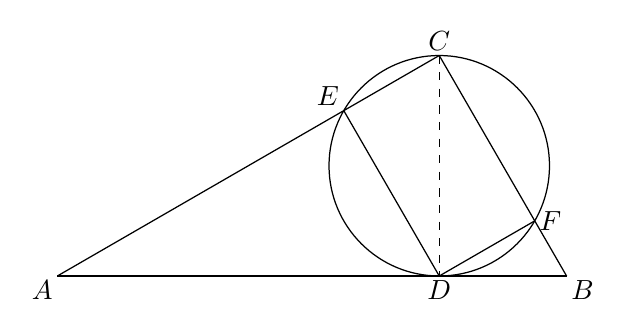
\begin{tikzpicture}[scale=1.4, line width=0.45pt,
  every node/.style={inner sep=1.5pt}]
  \coordinate (A) at (-3.464,-1);
  \coordinate (B) at (1.155,-1);
  \coordinate (C) at (0,1);
  \coordinate (D) at (0,-1);
  \coordinate (E) at (-0.866,0.5);
  \coordinate (F) at (0.866,-0.5);
  \draw (0,0) circle (1);
  \draw (A) -- (B);
  \draw (A) -- (C);
  \draw (B) -- (C);
  \draw (E) -- (D);
  \draw (D) -- (F);
  \draw[dashed] (C) -- (D);
  \node[anchor=north east] at (A) {$A$};
  \node[anchor=north west] at (B) {$B$};
  \node[anchor=south] at (C) {$C$};
  \node[anchor=north] at (D) {$D$};
  \node[anchor=south east] at (E) {$E$};
  \node[anchor=west] at (F) {$F$};
\end{tikzpicture}
\end{center}
\nopagebreak[4]
\end{question}
\begin{question}
\gkti{8}过原点 $O$ 作圆 $x^2+y^2-2x-4y+4=0$ 的任意割线交圆于 $P_1$、$P_2$ 两点，求 $P_1P_2$ 的中点 $P$ 的轨迹。

\end{question}